Los títulos de las secciones y subsecciones debieran verse como los aquí exhibidos. El interlineado entre los títulos de las secciones y subsecciones ya están preconfigurados en dicho template.
    \subsection{PRIMERA PÁGINA}   
        La primera página deberá contener un área predefinida para la información básica del trabajo de investigación, la de los autores y el resumen. El resumen deberá ser escrito en estilo cursiva. A continuación se presenta la correcta forma de citar una figura, como se observa en la figura 1.
        \begin{figure}[H]
            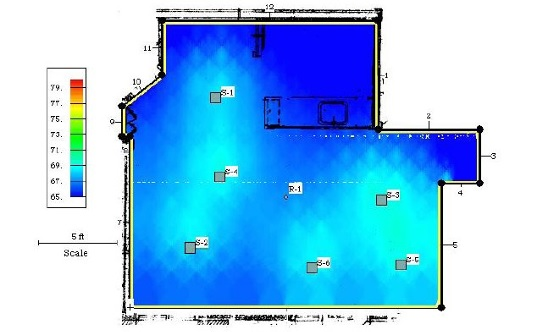
\includegraphics[width=7.6cm]{fig1} % Ojo con los margenes
            \caption{Planta del recinto y su distribución de SPL [dB].}
            \centering
        \end{figure}
        La información de la primera página deberá incluir:
            \begin{itemize}
                \item El título del trabajo.
                \item Los autores.
                \item Sus afiliaciones e información de contacto.
                \item Resumen (no más de 200 palabras).
                \item Palabras clave (Keywords).
            \end{itemize}
            